\subsubsection{Implementering}
Windows implementeres jævnfør designet ved at lave vinduer eller views, som implementerer view interfaces fra design af presentation-laget.

På figur~\ref{fig:wincreateuserandwinstatviewview} ses de klassediagrammet for de to views der præsenterer muligheden for at løse de to user stories, der er taget udgangspunkt i i starten af design og implementerings afsnittet.

Resultatet af implementeringen af WinStatView ses på følgende figur.

\begin{figure}
\centering
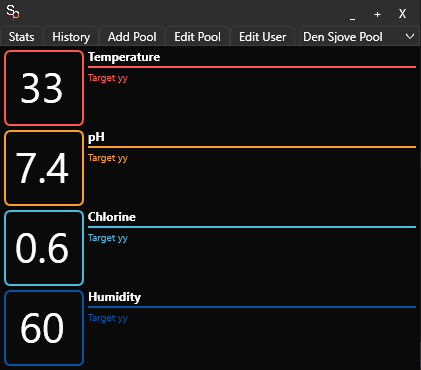
\includegraphics[width=0.5\linewidth]{figs/implementering/winstatview}
\caption{WinStatView resultat}
\label{fig:winstatview}
\end{figure}

I følgende kode er der udsnit fra view'et der præsenterer historisk data for brugeren. 

\begin{lstlisting}[caption=DisplayGraph, label=DisplayGraph]
private void DisplayGraph(Canvas historyCanvas, List<double> history, bool isPhOrChlorine)
{
...
var pointHeight = ((upperBound - history[i])) / (upperBound - lowerBound) * canvasHeight;
var pointWidth = (canvasWidth/(_pointsOnGraphs - 1))*i;
...
\end{lstlisting}

Koden er medbragt for at fremvise et view med mere dybde end de to på figur~\ref{fig:wincreateuserandwinstatviewview}.
Funktionen DisplayGraph() modtager historisk data og tegner en graf. 
På linje 9 og 10 udregnes punkterne på grafens højde relativt til størrelsen af grafen. At de udregnes relativt, gør at, grafen skalerer perfekt, når vinduet skaleres. 
Hver punkt i datamængden funktionen modtager tilføjes til et canvas, og linjes tegnes imellem.
Resultatet af DisplayGraph ses på følgende figur.

\begin{figure}
\centering
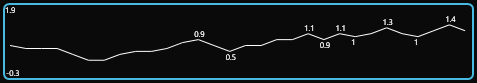
\includegraphics[width=0.4\linewidth]{figs/implementering/displaygraph}
\caption{Graf fra WinHistoryView}
\label{fig:displaygraph}
\end{figure}

For mere information se dokumentationen afsnit Windows Implementering.